\chapter{Neraca Momentum dan Energi dalam Aliran}\label{ch:b2:flow-balances}

Seorang pemadam kebakaran menahan tubuhnya melawan selang: air yang
berangkat pada tiga puluh meter tiap sekon mendorong balik dengan ratusan
newton, walaupun tak ada yang menyentuh corongnya selain air. Sebuah mesin
jet tergantung pada sayap dan menarik pesawat menembus langit dengan
melontarkan udara ke belakang. Sebuah penyiram taman berputar tanpa motor.
Dalam setiap hal sebuah fluida memasuki sebuah daerah, meninggalkannya
dengan momentum yang berbeda, dan selisihnya adalah sebuah gaya. Bab ini
menuliskan hukum mekanika --- momentum, momentum sudut, energi --- bukan
bagi massa fluida yang tetap melainkan bagi fluida yang menyeberangi
daerah tetap, yaitu \emph{\omterm{def:b2:flow-balances:cv}{sistem terbuka}}: bentuk yang dipakai insinyur
untuk mengukur turbin, roket, pompa dan pipa.

\section{Neraca bagi sistem terbuka}

\begin{definition}[Volume kendali; sistem terbuka]\label{def:b2:flow-balances:cv}
\index{volume kendali}\index{sistem terbuka}
Yang disebut \emph{volume kendali} (atau permukaan kendali) adalah daerah
ruang tetap $\Sigma$ yang dilewati aliran fluida; fluida di dalamnya pada
sembarang saat adalah \emph{sistem terbuka}, yang bertukar massa dengan
luarnya lewat lubang masuk dan lubang keluar $\Sigma$. Sistem tertutup
yang menuruti hukum Newton adalah fluida yang berada di dalam $\Sigma$
pada saat $t$, lalu diikuti sampai $t + \dd t$: ia lalu menempati $\Sigma$
dikurangi apa yang telah keluar ditambah apa yang telah masuk.
\end{definition}

\begin{theorem}[Neraca momentum dalam aliran tunak]\label{thm:b2:flow-balances:momentum}
\index{neraca momentum (aliran tunak)}\index{fluks momentum}
Untuk aliran tunak menembus sebuah \omterm{def:b2:flow-balances:cv}{volume kendali} dengan satu lubang
masuk (penampang $S_1$, kecepatan seragam $\vect v_1$) dan satu lubang
keluar ($S_2$, $\vect v_2$), dengan \omterm{def:b2:fluid-kinematics:flowrate}{debit massa} $D_m$ yang sama di keduanya,
\[
\sum\vect F_{\text{luar}} = D_m\,(\vect v_2 - \vect v_1) ,
\]
dengan $\sum\vect F_{\text{luar}}$ jumlah semua gaya luar pada
fluida di dalam $\Sigma$: berat, gaya dari dinding dan benda yang
bersentuhan dengannya, serta gaya tekanan pada penampang masuk dan
keluarnya ($P_1S_1\vect n_1$ yang mendorong ke dalam, $-P_2S_2\vect n_2$ di lubang keluarnya). Dengan
beberapa lubang masuk dan keluar, ruas kanannya adalah jumlah \omterm{thm:b2:flow-balances:momentum}{fluks
momentum} yang keluar $D_{m,i}\vect v_i$ dikurangi yang masuk.
\end{theorem}

\begin{proof}
Tinjaulah sistem tertutup $\mathcal S$ yang terdiri atas fluida dalam $\Sigma$ pada
saat $t$ ditambah lempeng $\delta m = D_m\dd t$ yang hendak masuk lewat $S_1$.
Pada $t + \dd t$ ia terdiri atas fluida dalam $\Sigma$ ditambah lempeng $\delta m$
yang telah keluar lewat $S_2$. Momentumnya beralih dari $\vect p_\Sigma(t) +
\delta m\,\vect v_1$ ke $\vect p_\Sigma(t + \dd t) + \delta m\,\vect v_2$; dalam aliran
tunak $\vect p_\Sigma$ tetap, jadi $\dd\vect p_{\mathcal S} = D_m\dd t\,(\vect v_2
- \vect v_1)$. Hukum kedua Newton bagi $\mathcal S$, yang gaya luarnya
(sampai orde pertama) adalah gaya pada fluida dalam $\Sigma$, memberi hasilnya.
\end{proof}

\begin{omfigure}
\begin{tikzpicture}[font=\small, x=1cm, y=1cm, >=Stealth]
  \draw[thick, omExo, dashed] (-2.2,-1.2) rectangle (2.6,1.2);
  \node[omExo, font=\footnotesize] at (-1.5,1.45) {volume kendali $\Sigma$};
  \draw[thick] (-3.4,0.6) -- (-2.2,0.6) .. controls (-1,0.6) and (0,1.0) .. (1.2,1.0) -- (2.6,1.0) -- (3.4,1.0);
  \draw[thick] (-3.4,-0.6) -- (-2.2,-0.6) .. controls (-1,-0.6) and (0,0.2) .. (1.2,0.2) -- (2.6,0.2) -- (3.4,0.2);
  \fill[omDef!25] (-3.4,-0.6) -- (-2.2,-0.6) .. controls (-1,-0.6) and (0,0.2) .. (1.2,0.2) -- (3.4,0.2) -- (3.4,1.0) -- (1.2,1.0) .. controls (0,1.0) and (-1,0.6) .. (-2.2,0.6) -- (-3.4,0.6) -- cycle;
  \draw[omDef, very thick] (-2.2,-0.6) -- (-2.2,0.6); \draw[omDef, very thick] (2.6,0.2) -- (2.6,1.0);
  \draw[omThm, very thick, ->] (-3.1,0) -- (-2.4,0) node[above, font=\footnotesize, pos=0.3] {$\vect v_1$};
  \draw[omThm, very thick, ->] (2.7,0.6) -- (3.3,0.6) node[above, font=\footnotesize, pos=0.3] {$\vect v_2$};
  \node[omDef, font=\footnotesize] at (-2.2,-0.95) {$S_1$, $P_1$}; \node[omDef, font=\footnotesize] at (2.6,-0.2) {$S_2$, $P_2$};
  \draw[omProp, very thick, ->] (0.3,-1.05) -- (0.3,-0.35) node[right, font=\footnotesize, pos=0.2] {$\vect F_{\text{dinding}}$};
  \node[font=\footnotesize] at (0.2,-1.7) {$\sum\vect F_{\text{luar}} = D_m(\vect v_2 - \vect v_1)$};
\end{tikzpicture}
\hfill
\begin{tikzpicture}[font=\small, x=1cm, y=1cm, >=Stealth]
  \begin{scope}
    \fill[pattern=north east lines] (1.2,-1.5) rectangle (1.4,1.5); \draw[thick] (1.2,-1.5) -- (1.2,1.5);
    \fill[omDef!25] (-2.2,-0.25) rectangle (1.2,0.25);
    \draw[omDef, thick] (-2.2,0.25) -- (1.2,0.25) (-2.2,-0.25) -- (1.2,-0.25);
    \draw[omDef, thick] (1.2,0.25) .. controls (0.9,0.7) and (0.8,1.0) .. (0.8,1.5);
    \draw[omDef, thick] (1.2,-0.25) .. controls (0.9,-0.7) and (0.8,-1.0) .. (0.8,-1.5);
    \draw[omThm, very thick, ->] (-1.6,0) -- (-0.6,0) node[above, font=\footnotesize] {$v$};
    \draw[omProp, very thick, ->] (1.4,0) -- (2.4,0) node[above, font=\footnotesize] {$F = D_mv$};
    \node[font=\footnotesize] at (0,-1.85) {pancaran pada dinding};
  \end{scope}
  \begin{scope}[xshift=5.4cm]
    \draw[thick] (0.2,0) .. controls (0.9,0) and (1.2,0.4) .. (1.2,1.0) .. controls (1.2,0.4) and (0.9,0) .. (0.2,0);
    \draw[thick, omExo] (0.25,0.0) .. controls (1.1,-0.05) and (1.35,0.55) .. (1.25,1.2);
    \draw[thick, omExo] (0.25,0.0) .. controls (1.1,0.05) and (1.35,-0.55) .. (1.25,-1.2);
    \fill[omDef!25] (-2.0,-0.2) rectangle (0.25,0.2);
    \draw[omDef, thick] (-2.0,0.2) -- (0.25,0.2) (-2.0,-0.2) -- (0.25,-0.2);
    \draw[omThm, very thick, ->] (-1.6,0) -- (-0.8,0) node[above, font=\footnotesize] {$v$};
    \draw[omDef, thick, ->] (0.4,0.3) .. controls (0.9,0.5) and (1.0,0.9) .. (0.6,1.2) node[left, font=\footnotesize] {$v - u$};
    \draw[omDef, thick, ->] (0.4,-0.3) .. controls (0.9,-0.5) and (1.0,-0.9) .. (0.6,-1.2);
    \draw[very thick, ->] (1.4,0.3) -- (2.1,0.3) node[right, font=\footnotesize] {$u$};
    \node[font=\footnotesize] at (0.2,-1.85) {mangkuk Pelton};
  \end{scope}
\end{tikzpicture}

{\small Kiri: sebuah \omterm{def:b2:flow-balances:cv}{volume kendali} dalam aliran tunak --- momentum
yang keluar lewat $S_2$ dikurangi yang masuk lewat $S_1$ sama dengan jumlah
gaya luar pada fluida di dalamnya, termasuk gaya tekanan pada kedua
penampangnya. Kanan: pancaran yang dihentikan dinding mendorongnya dengan
$D_mv$; pancaran yang dibalikkan mangkuk Pelton yang bergerak dengan $u$ mendorong
sampai $2D_m(v - u)$.}
\end{omfigure}

\begin{example}[Pancaran pada dinding; selang pemadam]\label{ex:b2:flow-balances:jet}
Sebuah pancaran berpenampang $s$ dan berkelajuan $v$ menumbuk dinding tegak lurus lalu
menyebar di atasnya: momentum keluar sepanjang pancarannya nol, jadi
dindingnya menerima $F = D_mv = \rho sv^2$ --- \qty{1.1}{kN} bagi pancaran \qty{5}{cm}
pada \qty{24}{m/s}. Dengan neraca yang sama yang diterapkan pada fluida dalam selang
dan corongnya, corongnya mendorong balik pemadamnya dengan $D_mv$:
\qty{20}{L/s} pada \qty{30}{m/s} memberi \qty{600}{N}, seberat seorang manusia.
Jika dindingnya mundur dengan $u$, hanya $D_m' = \rho s(v - u)$ yang mencapainya tiap satuan
waktu dan ia tiba dengan kelajuan nisbi $v - u$: $F = \rho s(v - u)^2$.
\end{example}

\begin{proposition}[Mangkuk Pelton; gaya dorong roket]\label{prop:b2:flow-balances:pelton}
\index{turbin Pelton}\index{gaya dorong}\index{persamaan roket}
(i) Sebuah pancaran berkelajuan $v$ dan berdebit massa $D_m$ dibalikkan sejauh
$180^\circ$ oleh sebuah mangkuk yang bergerak dengan $u$ searah pancarannya: gaya
pada mangkuknya adalah $F = 2D_m(v - u)$ (dengan $D_m$ debit yang sungguh-sungguh
dicegat mangkuk yang bergerak pada sebuah roda), dayanya $Fu$
maksimum untuk $u = v/2$ dan lalu sama dengan $\tfrac12D_mv^2$: seluruh
daya kinetik pancarannya. (ii) Sebuah roket bermassa $m(t)$ yang menyemburkan gas ke belakang dengan
kelajuan nisbi $v_e$ dan \omterm{def:b2:fluid-kinematics:flowrate}{debit massa} $D_m = -\dd m/\dd t$ merasakan
\omterm{prop:b2:flow-balances:pelton}{gaya dorong} $F = D_mv_e$; dalam ruang bebas kelajuannya bertambah sebesar
$\Delta v = v_e\ln(m_0/m_1)$ (\omterm{prop:b2:flow-balances:pelton}{persamaan roket} Tsiolkovsky); di bawah gravitasi,
$m\,\dd v/\dd t = D_mv_e - mg$.
\end{proposition}

\begin{proof}
(i) Dalam kerangka mangkuknya pancarannya tiba dengan $v - u$ dan berangkat dengan
$-(v - u)$; neraca momentumnya memberi $2D_m(v - u)$ (mangkuknya
sempurna: tanpa rugi kelajuan nisbi). Dayanya $2D_mu(v - u)$, maksimum pada
$u = v/2$. (ii) Momentum roket ditambah gas yang disemburkan dalam $\dd t$: $(m + \dd m)
(v + \dd v) + (-\dd m)(v - v_e) = mv$ dalam ruang bebas, jadi $m\,\dd v = -\dd m\,v_e$
dan $v_1 - v_0 = v_e\ln(m_0/m_1)$; dengan gravitasi momentum totalnya berubah
sebesar $-mg\,\dd t$.
\end{proof}

\begin{example}[Sebuah peluncur]\label{ex:b2:flow-balances:rocket}
Tingkat pertama: $D_m = \qty{2500}{kg/s}$ pada $v_e = \qty{3000}{m/s}$: \omterm{prop:b2:flow-balances:pelton}{gaya dorongnya}
\qty{7.5}{MN}, yang mengangkat roket \qty{600}{t} dengan $7.5 \times 10^6/6 \times 10^5 - g
= \qty{2.7}{m/s^2}$ dari landasannya. Membakar \qty{500}{t} dalam \qty{200}{s} memberi
$\Delta v = 3000\ln6 - 9.81 \times 200 = 5400 - 2000 = \qty{3.4}{km/s}$ --- rugi
gravitasinya adalah sebab peluncur menanjak cepat, dan logaritmanya sebab mereka
dibuat bertingkat.
\end{example}

\begin{example}[Gaya pada belokan pipa]\label{ex:b2:flow-balances:bend}
Air pada $P$ dan $v$ dalam pipa berpenampang $S$ membelok sejauh $90^\circ$. Neraca
pada fluida dalam sikunya: $\vect F_{\text{dinding}} + PS\vect e_x - PS
\vect e_y = D_m(v\vect e_y - v\vect e_x)$, jadi dindingnya mendorong fluidanya dengan
$\vect F_{\text{dinding}} = -(PS + \rho Sv^2)(\vect e_x - \vect e_y)$ dan fluidanya
mendorong sikunya ke luar dengan $(PS + \rho Sv^2)\sqrt2$. Untuk $D = \qty{20}{cm}$,
$P = \qty{3}{bar}$, $v = \qty{3}{m/s}$: $PS = \qty{9.4}{kN}$, $\rho Sv^2 = \qty{0.28}{kN}$,
gayanya \qty{13.7}{kN} sepanjang garis baginya --- suku tekanannya menguasai,
dan itulah yang ditahan blok jangkar sebuah pipa saluran.
\end{example}

\section{Momentum sudut: turbin dan penyiram}

\begin{theorem}[Neraca momentum sudut; persamaan turbin Euler]\label{thm:b2:flow-balances:angular}
\index{neraca momentum sudut (aliran)}\index{persamaan turbin Euler}
Dalam aliran tunak, momen total terhadap sebuah titik $O$ dari gaya luar
pada fluida dalam $\Sigma$ sama dengan \omterm{thm:b2:flow-balances:momentum}{fluks momentum} sudut yang
keluar dikurangi yang masuk: $\sum\vect{\mathcal M}_O = D_m(\vect r_2\wedge\vect v_2 - \vect r_1
\wedge\vect v_1)$. Untuk mesin berputar (turbin atau pompa) bersumbu $Oz$,
dengan fluidanya masuk pada jari-jari $r_1$ berkecepatan azimut
$v_{\theta1}$ dan keluar pada $r_2$ dengan $v_{\theta2}$, momen gaya yang dikerahkan
fluidanya pada rotornya dan daya yang diserahkannya adalah
\[
\Gamma = D_m(r_1v_{\theta1} - r_2v_{\theta2}) , \qquad
\mathcal P = \Gamma\omega = D_m\omega(r_1v_{\theta1} - r_2v_{\theta2}) .
\]
Sebuah turbin mengambil pusaran keluar dari fluidanya; sebuah pompa memasukkannya.
\end{theorem}

\begin{proof}
Argumen sistem tertutup yang sama dengan $\vect r\wedge\vect v$ menggantikan
$\vect v$. Momen gaya pada rotornya adalah lawan dari momen gaya
rotornya pada fluidanya; gaya tekanan pada permukaan masuk dan keluarnya
(yang merupakan permukaan putar) tak bermomen terhadap
sumbunya.
\end{proof}

\begin{example}[Penyiram halaman]\label{ex:b2:flow-balances:sprinkler}
Dua lengan sepanjang $R$ menyemburkan air secara tangensial dengan kelajuan nisbi
$w$; penyiramnya berputar dengan $\omega$. Air masuk pada sumbunya tanpa
momentum sudut dan keluar dengan $r v_\theta = R(w - R\omega)$ (kelajuan
azimut mutlaknya $w - R\omega$, berlawanan dengan putarannya): momen gaya pada
lengannya adalah $D_mR(w - R\omega)$. Dalam keadaan diam nilainya $D_mRw$; tanpa gesekan
penyiramnya dipercepat sampai $R\omega = w$ --- airnya berangkat dengan kelajuan
mutlak nol dan momen gayanya lenyap; dengan momen gesek
$\Gamma_f$ ia menetap pada $\omega = (w - \Gamma_f/D_mR)/R$.
\end{example}

\begin{omfigure}
\begin{tikzpicture}[font=\small, x=1cm, y=1cm, >=Stealth]
  \begin{scope}
    \fill (0,0) circle (2pt);
    \draw[thick] (-1.8,0.12) rectangle (1.8,-0.12);
    \draw[thick] (1.8,-0.12) -- (1.8,0.5) (1.55,-0.12) -- (1.55,0.5);
    \draw[thick] (-1.8,0.12) -- (-1.8,-0.5) (-1.55,0.12) -- (-1.55,-0.5);
    \draw[omThm, very thick, ->] (1.68,0.5) -- (1.68,1.4) node[right, font=\footnotesize] {$w$};
    \draw[omThm, very thick, ->] (-1.68,-0.5) -- (-1.68,-1.4) node[left, font=\footnotesize] {$w$};
    \draw[omDef, ->, thick] (0.7,-0.6) arc[start angle=-40, end angle=-140, radius=0.9] node[midway, below, font=\footnotesize] {$\omega$};
    \node[font=\footnotesize] at (0,-2.0) {$\Gamma = D_mR(w - R\omega)$};
  \end{scope}
  \begin{scope}[xshift=6.6cm]
    \draw[omExo, thick] (0,0) circle (1.6); \draw[omExo, thick] (0,0) circle (0.6);
    \foreach \a in {0,45,...,315} \draw[omExo, thick] ({0.6*cos(\a)},{0.6*sin(\a)}) .. controls ({1.0*cos(\a+25)},{1.0*sin(\a+25)}) .. ({1.6*cos(\a+40)},{1.6*sin(\a+40)});
    \draw[omThm, very thick, ->] (1.9,-0.9) -- (1.55,-0.35) node[right, font=\footnotesize, pos=0.1] {$\vect v_1$};
    \draw[omThm, very thick, ->] (0.42,0.42) -- (0.0,0.55);
    \node[omThm, font=\footnotesize] at (0.15,0.85) {$\vect v_2$};
    \draw[omDef, ->, thick] (1.0,1.73) arc[start angle=60, end angle=130, radius=2.0] node[midway, above, font=\footnotesize] {$\omega$};
    \node[font=\footnotesize] at (0,-2.15) {$\Gamma = D_m(r_1v_{\theta1} - r_2v_{\theta2})$};
  \end{scope}
\end{tikzpicture}

{\small Kiri: penyiram halaman --- air berangkat dari lengannya secara tangensial
dengan kelajuan nisbi $w$; momentum sudut yang keluar memutar lengannya
ke arah sebaliknya. Kanan: sebuah turbin beraliran masuk radial (roda jalan Francis dilihat
sepanjang sumbunya): fluidanya masuk di peleknya dengan pusaran besar dan
keluar dekat sumbunya dengan pusaran kecil; selisih \omterm{thm:b2:flow-balances:momentum}{fluks momentum}
sudutnya adalah momen gaya pada roda jalannya.}
\end{omfigure}

\section{Neraca energi: pompa, turbin dan rugi-rugi}

\begin{theorem}[Neraca energi mekanik sebuah aliran tunak]\label{thm:b2:flow-balances:energy}
\index{neraca energi (aliran)}\index{daya hidraulik}\index{tinggi tekan}
Untuk fluida tak termampatkan dalam aliran tunak menembus sebuah mesin (pompa atau
turbin) antara lubang masuk 1 dan lubang keluar 2, dengan $\mathcal P_u$
daya mekanik yang diserahkan kepada fluidanya oleh bagian yang bergerak (positif bagi
pompa, negatif bagi turbin) dan $\mathcal P_{\text{les}} \ge 0$ daya
yang dilesapkan \omterm{def:b2:viscous-flows:viscosity}{kekentalannya},
\[
D_V\Bigl[\bigl(P_2 + \tfrac12\rho v_2^2 + \rho gz_2\bigr) - \bigl(P_1 + \tfrac12\rho v_1^2
+ \rho gz_1\bigr)\Bigr] = \mathcal P_u - \mathcal P_{\text{les}} .
\]
Dibagi $\rho gD_V$ ia memberi neracanya dalam \emph{\omterm{thm:b2:flow-balances:energy}{tinggi tekan}} (meter
fluida): $H_2 - H_1 = H_{\text{pompa}} - H_{\text{rugi}}$, dengan $H = P/\rho g +
v^2/2g + z$. Bagi \omterm{def:b2:euler-bernoulli:perfect}{fluida sempurna} tanpa mesin ini adalah Bernoulli;
\emph{\omterm{thm:b2:flow-balances:energy}{daya hidraulik}} sebuah pompa yang menaikkan \omterm{thm:b2:flow-balances:energy}{tinggi tekan} sebesar $H_{\text{pompa}}$ adalah
$\rho gD_VH_{\text{pompa}}$.
\end{theorem}

\begin{proof}
Teorema energi kinetik bagi sistem tertutup pada bukti
\cref{thm:b2:flow-balances:momentum}: dalam $\dd t$ energi kinetiknya
berubah sebesar $D_m\dd t\,(v_2^2 - v_1^2)/2$; usaha yang dilakukan padanya adalah usaha
gravitasi, $-D_m\dd t\,g(z_2 - z_1)$, usaha gaya tekanan pada muka ujung
yang bergerak, $(P_1S_1v_1 - P_2S_2v_2)\dd t = (P_1 - P_2)D_V\dd t$, usaha
bagian yang bergerak, $\mathcal P_u\dd t$, dan usaha gaya kental dalamnya,
$-\mathcal P_{\text{les}}\dd t$ (dindingnya, yang diam, tak melakukan usaha). Bagilah dengan
$\dd t$.
\end{proof}

\begin{example}[Mengukur sebuah pompa]\label{ex:b2:flow-balances:pump}
Air hendak diangkat \qty{30}{m} dengan \qty{20}{L/s} menembus \qty{100}{m}
pipa \qty{10}{cm} ($\lambda = 0.02$): $v = \qty{2.5}{m/s}$, rugi \omterm{thm:b2:flow-balances:energy}{tinggi tekannya} $\lambda(L/D)
v^2/2g = 0.02 \times 1000 \times 0.32 = \qty{6.4}{m}$, \omterm{thm:b2:flow-balances:energy}{tinggi tekan} kinetik keluarnya
\qty{0.32}{m}: $H_{\text{pompa}} = \qty{36.7}{m}$, \omterm{thm:b2:flow-balances:energy}{daya hidrauliknya} $\rho gD_VH =
\qty{7.2}{kW}$, dan \qty{10}{kW} listrik pada efisiensi $70\%$.
Tekanan di lubang keluar pompanya adalah $\rho gH_{\text{pompa}} \approx \qty{3.6}{bar}$ di atas
lubang masuknya.
\end{example}

\begin{proposition}[Pelebaran mendadak: rugi Borda--Carnot]\label{prop:b2:flow-balances:borda}
\index{rugi Borda--Carnot}\index{rugi tinggi tekan setempat}
Ketika pipa berpenampang $S_1$ membuka mendadak ke dalam pipa berpenampang $S_2
> S_1$, pancarannya menyebar dalam daerah turbulen dan tekanannya
\emph{naik} di hilirnya, tetapi lebih kecil daripada yang dikatakan Bernoulli:
energi mekanik yang hilang tiap satuan volume adalah
\[
\Delta P_{\text{rugi}} = \tfrac12\rho(v_1 - v_2)^2 ,
\]
yaitu energi kinetik kecepatan nisbi yang ``hilang''. Aliran yang berangkat dari
sebuah pipa ke dalam tangki besar ($v_2 \to 0$) kehilangan seluruh energi kinetiknya.
\end{proposition}

\begin{proof}
Neraca momentum pada fluida antara pelebarannya dan sebuah penampang di
hilirnya tempat alirannya kembali seragam; percobaan memperlihatkan
tekanan pada dinding cincin di pelebarannya sama dengan $P_1$ (pancarannya belum
menyebar). Jadi $(P_1 - P_2)S_2 = D_m(v_2 - v_1) = \rho S_2v_2(v_2 -
v_1)$, yakni $P_2 - P_1 = \rho v_2(v_1 - v_2)$. Bernoulli akan memberi
$\tfrac12\rho(v_1^2 - v_2^2)$; selisihnya adalah $\tfrac12\rho(v_1 - v_2)^2$.
\end{proof}

\begin{omfigure}
\begin{tikzpicture}[font=\small, x=1cm, y=1cm, >=Stealth]
  \draw[thick] (-3,0.5) -- (0,0.5) -- (0,1.2) -- (3.5,1.2);
  \draw[thick] (-3,-0.5) -- (0,-0.5) -- (0,-1.2) -- (3.5,-1.2);
  \fill[omDef!15] (-3,-0.5) rectangle (0,0.5); \fill[omDef!15] (0,-1.2) rectangle (3.5,1.2);
  \draw[omDef, dashed] (0,0.5) .. controls (1.2,0.6) and (2.0,1.1) .. (2.8,1.2);
  \draw[omDef, dashed] (0,-0.5) .. controls (1.2,-0.6) and (2.0,-1.1) .. (2.8,-1.2);
  \foreach \y in {0.75,1.0} { \draw[omProp, ->] (0.9,\y) arc[start angle=90, end angle=-200, radius=0.12]; }
  \foreach \y in {-0.75,-1.0} { \draw[omProp, ->] (0.9,\y) arc[start angle=-90, end angle=200, radius=0.12]; }
  \draw[omThm, very thick, ->] (-2.4,0) -- (-1.4,0) node[above, font=\footnotesize] {$v_1$, $P_1$};
  \draw[omThm, very thick, ->] (2.2,0) -- (3.0,0) node[above, font=\footnotesize] {$v_2$, $P_2$};
  \node[font=\footnotesize] at (0.3,-1.6) {$\Delta P_{\text{rugi}} = \tfrac12\rho(v_1 - v_2)^2$};
\end{tikzpicture}
\hfill
\begin{tikzpicture}
\begin{axis}[omaxis, axis x line=bottom, axis y line=left, width=6.4cm, height=4.3cm,
    xlabel={$S_1/S_2$}, ylabel={bagian dari $\tfrac12\rho v_1^2$}, xmin=0, xmax=1, ymin=0, ymax=1.05,
    xlabel style={at={(axis description cs:0.5,-0.12)}, anchor=north},
    ylabel style={at={(axis description cs:-0.14,0.5)}, rotate=90, anchor=south},
    xtick={0,0.5,1}, ytick={0,0.5,1}, samples=60,
    legend style={font=\scriptsize, at={(0.97,0.95)}, anchor=north east, draw=none, fill=none}]
  \addplot[omThm, thick, domain=0:1] {(1-x)^2};
  \addplot[omDef, thick, domain=0:1] {2*x*(1-x)};
  \legend{hilang, tekanan terpulihkan}
\end{axis}
\end{tikzpicture}

{\small Kiri: sebuah pelebaran mendadak --- pancarannya menyebar dalam daerah
mati yang turbulen dan sebagian energi kinetiknya dilesapkan. Kanan:
bagian energi kinetik hulunya yang hilang dan yang terpulihkan sebagai
tekanan, terhadap nisbah penampangnya; ruginya terbesar bagi pancaran
ke dalam tangki.}
\end{omfigure}

\begin{method}[Menyusun sebuah neraca]\label{met:b2:flow-balances:method}
(1) Gambarlah \omterm{def:b2:flow-balances:cv}{volume kendalinya}: batasnya sebaiknya memotong alirannya hanya
di tempat kecepatan dan tekanannya diketahui atau dicari (penampang seragam,
pancaran bebas pada $P_0$, permukaan bebas). (2) Daftarlah gaya luar pada
\emph{fluida di dalamnya}: berat, gaya dinding (yang tak diketahui, biasanya sasarannya),
tekanan pada penampang yang dipotongnya. (3) Tuliskanlah \omterm{thm:b2:flow-balances:momentum}{fluks momentum} yang keluar dikurangi yang masuk;
bagi bagian yang bergerak, bekerjalah dalam kerangka bagian itu jika alirannya tunak
di sana. (4) Untuk momen gaya, pakailah neraca momentum sudut; untuk daya,
neraca energi dalam \omterm{thm:b2:flow-balances:energy}{tinggi tekan}. (5) Gaya pada dindingnya adalah lawan gaya
dindingnya pada fluidanya; tambahkanlah tekanan atmosfer yang bekerja pada
sisi luar perangkatnya jika gaya total pada perangkatnya yang dicari.
\end{method}

\section{Latihan}

\begin{exercise}[$\star$]\label{exo:b2:flow-balances:1}
Sebuah selang pemadam menyerahkan \qty{25}{L/s} lewat corong berdiameter
\qty{3.0}{cm}. Tentukanlah kelajuan keluarnya; gaya reaksi pada corongnya; gaya pancarannya
pada dinding yang ditumbuknya tegak lurus; pada dinding yang mundur dengan \qty{10}{m/s}.
\end{exercise}

\begin{exercise}[$\star$]\label{exo:b2:flow-balances:2}
Sebuah mesin roket menyemburkan \qty{250}{kg/s} pada \qty{3.0}{km/s}. Tentukanlah \omterm{prop:b2:flow-balances:pelton}{gaya dorongnya}; percepatan
awal roket \qty{60}{t}; percepatannya ketika \qty{40}{t}
propelan telah terbakar; kelajuan yang diperoleh sesudah pembakaran itu (dalam ruang bebas, lalu
dengan gravitasi, berdurasi \qty{160}{s}).
\end{exercise}

\begin{exercise}[$\star$]\label{exo:b2:flow-balances:3}
Air mengalir dengan \qty{2.0}{m/s} pada \qty{4.0}{bar} dalam pipa \qty{15}{cm} yang
membelok sejauh \qty{90}{\degree}. Tentukanlah gaya yang dikerahkan airnya pada sikunya
(besar dan arahnya); bagian mana yang datang dari tekanannya, bagian mana
dari perubahan momentumnya? Siku yang sama dengan pipanya terbuka ke udara tepat
sesudah belokannya.
\end{exercise}

\begin{exercise}[$\star$]\label{exo:b2:flow-balances:4}
Sebuah mesin jet di landasan uji menelan \qty{80}{kg/s} udara yang diam lalu
membuangnya pada \qty{550}{m/s} (massa bahan bakarnya diabaikan). Tentukanlah \omterm{prop:b2:flow-balances:pelton}{gaya dorongnya}. Dalam terbang
pada \qty{240}{m/s}, dengan kelajuan buang yang sama nisbi terhadap mesinnya: \omterm{prop:b2:flow-balances:pelton}{gaya dorong},
daya propulsi, dan daya kinetik yang diberikan kepada udaranya dalam kerangka
mesinnya; efisiensi propulsinya.
\end{exercise}

\begin{exercise}[$\star\star$]\label{exo:b2:flow-balances:5}
\emph{Roda Pelton.} Sebuah pancaran \qty{0.50}{m^3/s} pada \qty{60}{m/s} menumbuk
mangkuk sebuah roda berjari-jari \qty{0.80}{m}. (a) Gaya dan daya pada
mangkuknya pada kelajuan mangkuk $u$ (pembelokan $180^\circ$ yang sempurna); $u$ optimum
dan laju putar yang bersesuaian dalam rpm. (b) Daya dan efisiensinya
pada optimumnya. (c) Mangkuk sungguhan membelokkan pancarannya sejauh \qty{165}{\degree}:
gaya dan daya pada $u = v/2$; efisiensinya. (d) Momen gaya pada optimumnya;
apa yang terjadi pada momen gayanya saat berhenti dan pada kelajuan lepas kendalinya?
\end{exercise}

\begin{exercise}[$\star\star$]\label{exo:b2:flow-balances:6}
\emph{Penyiram.} Dua lengan \qty{15}{cm} berujung corong \qty{3.0}{mm};
alirannya total \qty{0.20}{L/s}. (a) Kelajuan keluar nisbinya. (b) Momen gaya dalam
keadaan diam. (c) Laju putarnya dengan momen gesek \omterm{def:b2:rigid-body-mechanics:pivot}{bantalan} sebesar
\qty{5.0e-3}{N.m}; laju batasnya tanpa gesekan. (d) Kelajuan mutlak
air yang berangkat, dalam tiap hal.
\end{exercise}

\begin{exercise}[$\star\star$]\label{exo:b2:flow-balances:7}
\emph{Melayang di tempat.} Sebuah helikopter \qty{2.0}{t} melayang di tempat dengan rotor
berdiameter \qty{10}{m}. Modelkanlah rotornya sebagai cakram yang menerima udara diam
lalu mendorongnya turun menembus kelajuan seragam $v_i$ di cakramnya, $2v_i$ jauh
di bawahnya (terimalah faktor 2 itu). (a) \omterm{prop:b2:flow-balances:pelton}{Gaya dorongnya} dalam $\rho$, $A$, $v_i$;
nilai $v_i$. (b) Daya yang diberikan kepada udaranya (daya kinetiknya jauh
di bawah). (c) Mengapa rotor yang lebih besar menuntut daya lebih kecil? (d) Perhitungan
yang sama bagi sebuah dron \qty{1}{kg} dengan empat baling-baling \qty{25}{cm};
bandingkanlah nisbah daya terhadap beratnya.
\end{exercise}

\begin{exercise}[$\star\star$]\label{exo:b2:flow-balances:8}
\emph{Pelebaran mendadak.} Air pada \qty{4.0}{m/s} dalam pipa \qty{5}{cm} memasuki
pipa \qty{10}{cm}. (a) Kelajuan di hilirnya; kenaikan tekanannya menurut
Bernoulli dan menurut Borda--Carnot; ruginya dalam pascal dan dalam meter
\omterm{thm:b2:flow-balances:energy}{tinggi tekan}. (b) Pelebaran yang sama dibuat berangsur (sebuah difuser) memulihkan $80\%$
kenaikan Bernoullinya: ruginya. (c) Ruginya ketika pipa \qty{5}{cm} mencurah
ke dalam tangki besar. (d) Daya yang hilang dalam hal (a) dan (c) pada aliran yang diberikan.
\end{exercise}

\begin{exercise}[$\star\star$]\label{exo:b2:flow-balances:9}
Sebuah pompa menyedot air dari sumur \qty{5.0}{m} di bawahnya lalu menyerahkan
\qty{10}{L/s} ke tangki \qty{25}{m} di atasnya menembus \qty{60}{m} pipa \qty{6}{cm}
($\lambda = 0.025$, ditambah rugi setempat $2\,v^2/2g$ bagi sambungannya).
(a) Kelajuan dan rugi-ruginya. (b) \omterm{thm:b2:flow-balances:energy}{Tinggi tekan} pompanya dan \omterm{thm:b2:flow-balances:energy}{daya hidrauliknya}; daya porosnya
pada efisiensi $65\%$. (c) Tekanan di lubang masuk pompanya (sisi isap) dan
lubang keluarnya. (d) Tekanan uap airnya \qty{2.3}{kPa}: tinggi maksimum
pompanya di atas sumurnya.
\end{exercise}

\begin{exercise}[$\star\star\star$]\label{exo:b2:flow-balances:10}
\emph{Roket air.} Sebuah botol \qty{2.0}{L} berisi \qty{1.0}{L} air dan
udara pada \qty{5.0}{bar} (mutlak); corongnya berdiameter \qty{2.2}{cm};
botol kosongnya \qty{0.10}{kg}. (a) Kelajuan keluar awalnya (Bernoulli, dengan permukaan
airnya diam) dan \omterm{prop:b2:flow-balances:pelton}{gaya dorongnya}; percepatan awalnya. (b) Ketika airnya keluar
udaranya memuai secara isotermal: tekanan dan kelajuan keluarnya ketika separuh
airnya habis. (c) Perkirakanlah durasi pembakarannya dan kelajuan yang dicapainya
(abaikanlah gravitasi dan seretannya, perlakukanlah \omterm{prop:b2:flow-balances:pelton}{gaya dorongnya} sebagai nilai reratanya). (d)
Apa yang dilakukan botol kosongnya setelah airnya habis, dan mengapa sedikit
air (bukan banyak) memberi ketinggian terbaik?
\end{exercise}

\begin{exercise}[$\star\star\star$]\label{exo:b2:flow-balances:11}
\emph{Turbin Francis.} Air memasuki roda jalan pada $r_1 = \qty{1.0}{m}$ dengan
$v_{\theta1} = \qty{20}{m/s}$ dan keluar pada $r_2 = \qty{0.50}{m}$ tanpa pusaran;
alirannya \qty{30}{m^3/s}; putarannya \qty{150}{rpm}. (a) Momen gaya dan dayanya. (b)
\omterm{thm:b2:flow-balances:energy}{Tinggi tekan} yang tersedot, $H = \mathcal P/\rho gD_V$. (c) Jika roda jalannya berjalan pada
\qty{200}{rpm} dengan kecepatan masuk yang sama dan pusaran keluarnya menjadi
$v_{\theta2} = \qty{3}{m/s}$ searah putarannya: dayanya dan
bagian \omterm{thm:b2:flow-balances:energy}{tinggi tekannya} yang berubah menjadi pusaran keluar yang tak berguna. (d) Mengapa
roda Pelton dipakai bagi \omterm{thm:b2:flow-balances:energy}{tinggi tekan} besar dan aliran kecil, dan Francis untuk
kebalikannya?
\end{exercise}

\begin{exercise}[$\star\star\star$]\label{exo:b2:flow-balances:12}
\emph{Loncatan hidraulik.} Dalam saluran mendatar berlebar satuan, air
sedalam $h_1$ yang mengalir dengan $v_1$ meloncat mendadak menjadi kedalaman $h_2$ dan kelajuan
$v_2$ (undakan berbuih di bawah sebuah bendung atau dalam bak cuci piring). (a) Kekekalan
massanya. (b) Neraca momentum pada fluida antara kedua sisi
loncatannya, dengan tekanannya hidrostatik di kedua sisinya: tunjukkanlah
$\tfrac12gh_1^2 + v_1^2h_1 = \tfrac12gh_2^2 + v_2^2h_2$. (c) Simpulkanlah $h_2/h_1 =
\tfrac12\bigl(-1 + \sqrt{1 + 8\,\mathrm{Fr}_1^2}\bigr)$ dengan $\mathrm{Fr}_1 =
v_1/\sqrt{gh_1}$ (bilangan Froude); sebuah loncatan menuntut $\mathrm{Fr}_1 > 1$. (d)
\omterm{thm:b2:flow-balances:energy}{Tinggi tekan} yang hilang dalam loncatannya, $\Delta H = (h_2 - h_1)^3/4h_1h_2$; angkanya untuk $h_1 =
\qty{0.20}{m}$, $v_1 = \qty{4.0}{m/s}$, serta daya yang dilesapkan tiap meter
lebarnya.
\end{exercise}

\begin{omfigure}
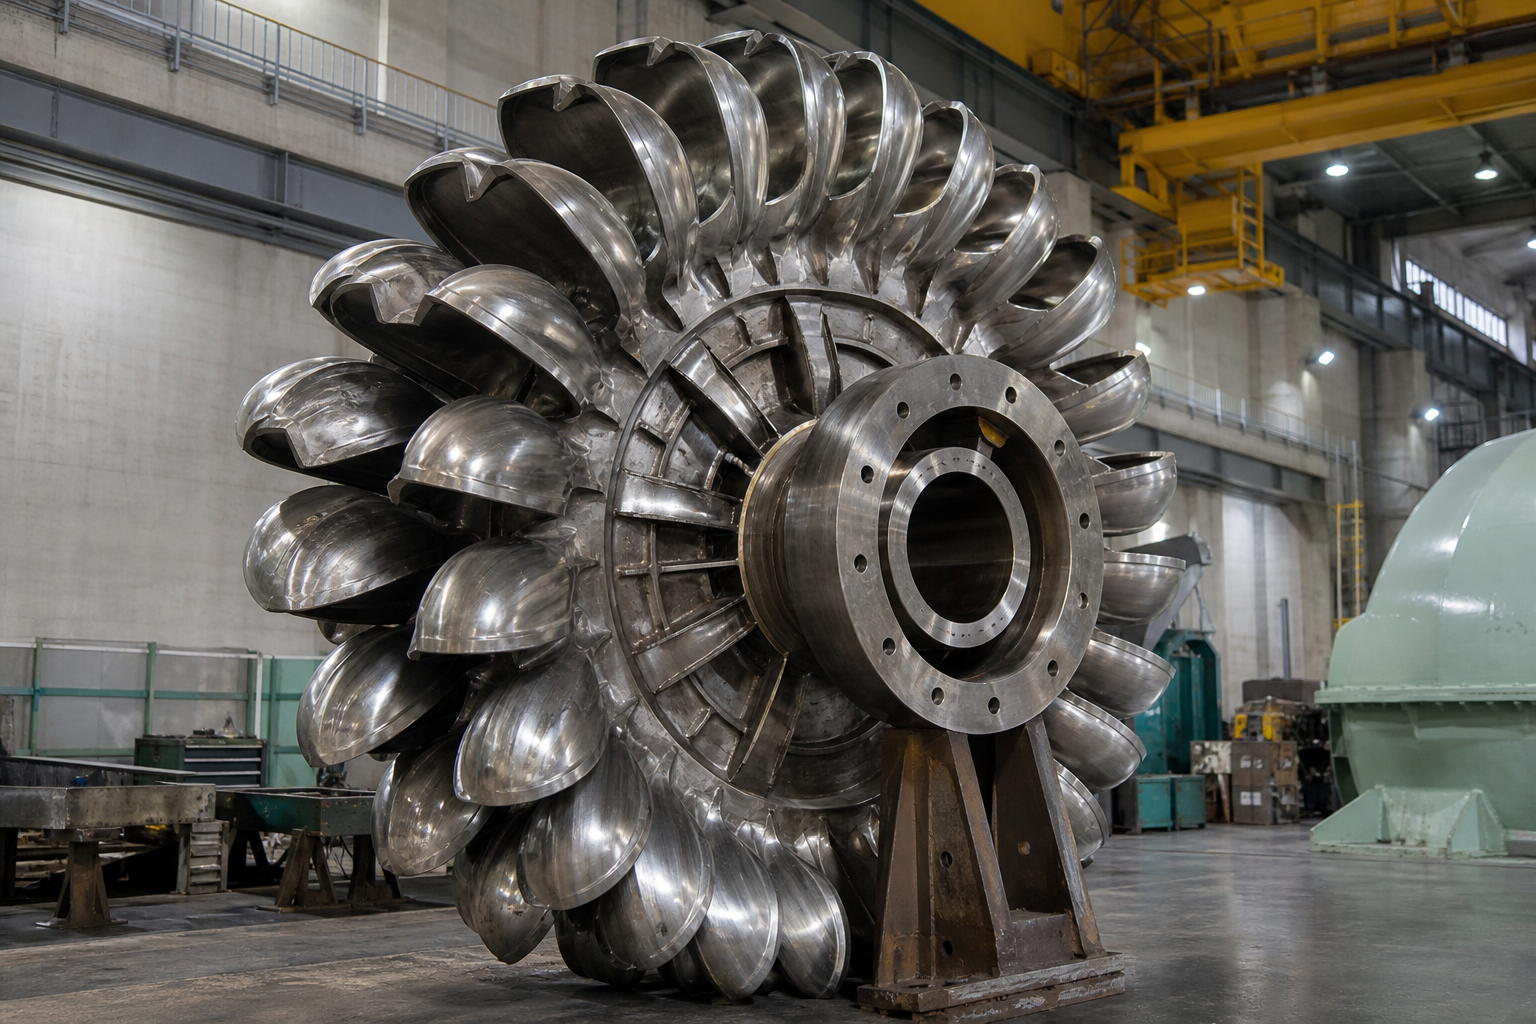
\includegraphics[width=0.58\linewidth]{images/book4/ai/b4-05-pelton-wheel.png}

{\small Roda jalan sebuah \omterm{prop:b2:flow-balances:pelton}{turbin Pelton}: tiap mangkuk membalikkan pancarannya hampir sejauh $180^\circ$, dan perubahan momentum airnya adalah gaya pada rodanya.}
\end{omfigure}

\begin{omfigure}
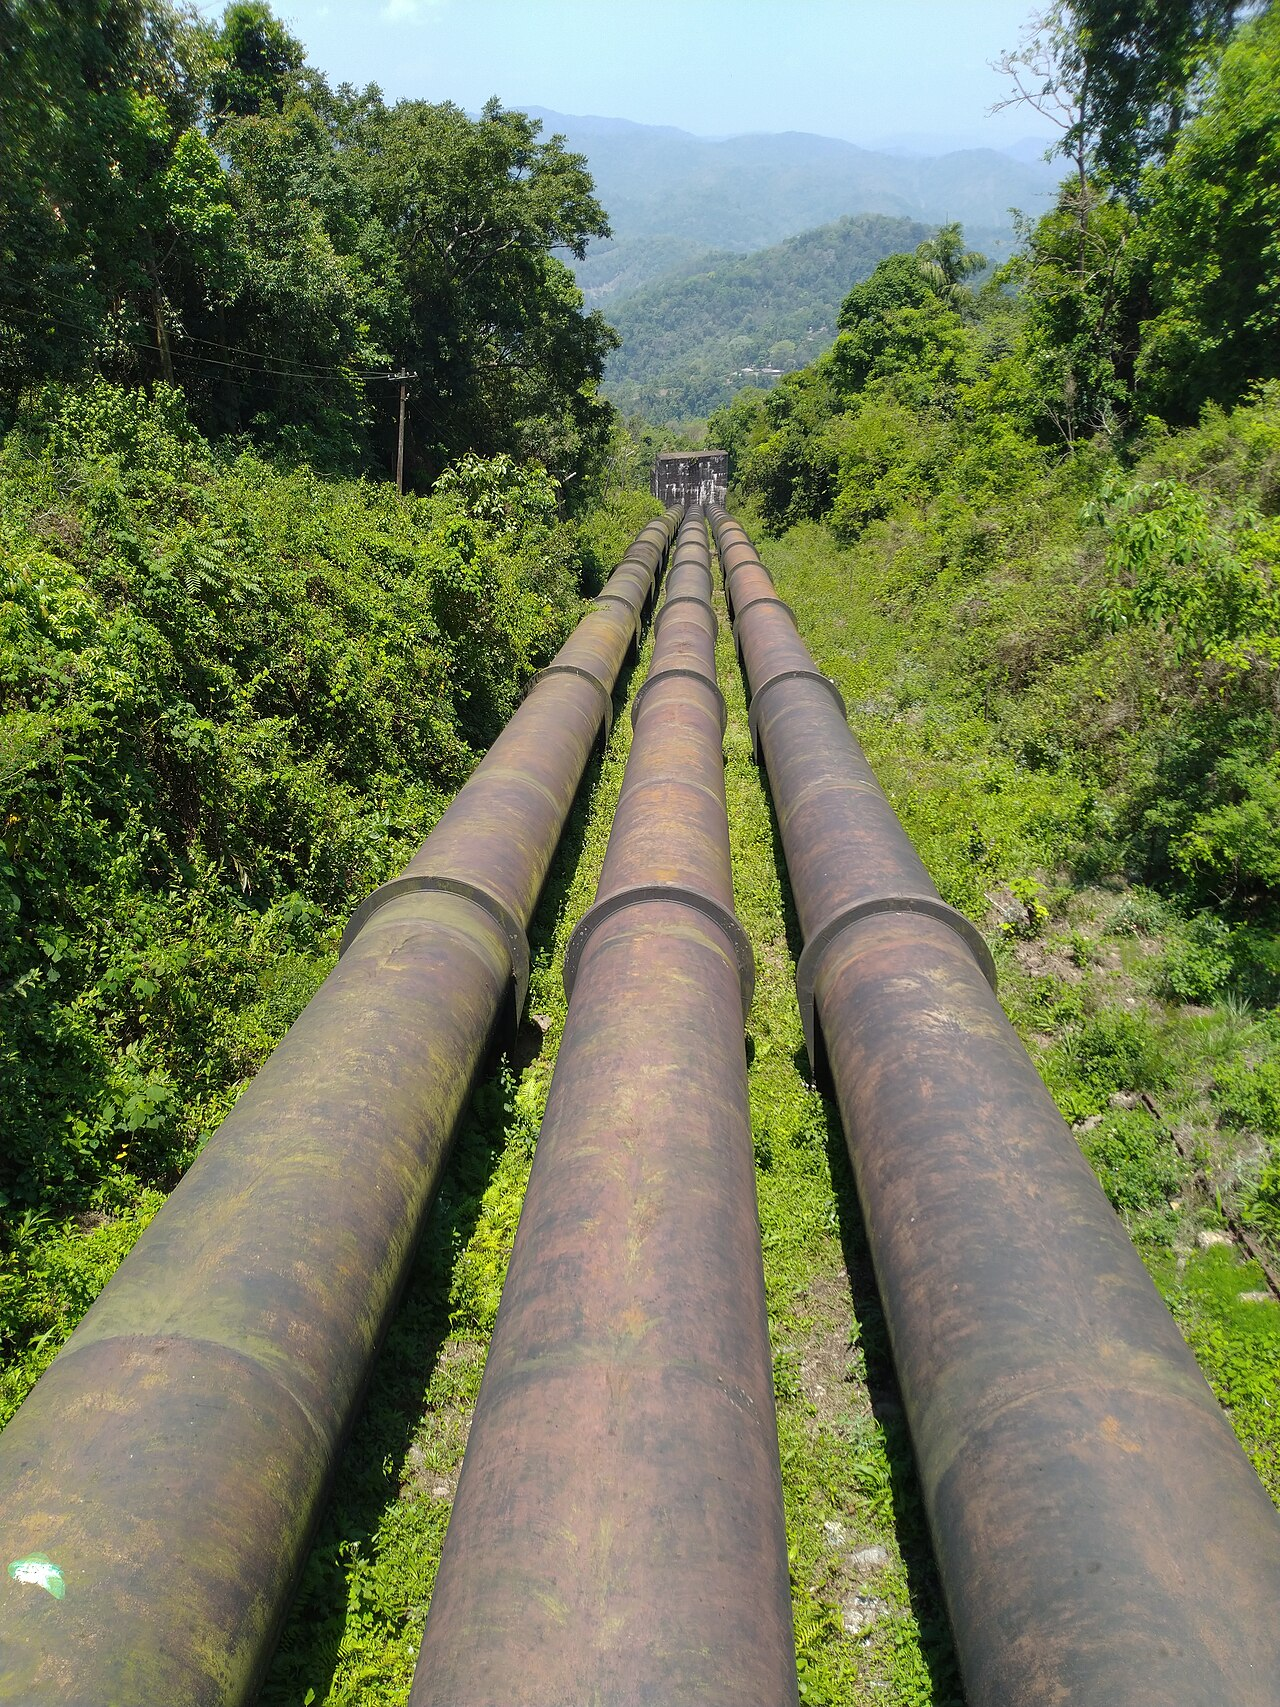
\includegraphics[width=0.42\linewidth]{images/book4/penstock-sabarigiri.jpg}

{\small Pipa pesat sebuah pembangkit listrik tenaga air menyuapi turbin di bawahnya: neraca momentum pancarannya pada mangkuk roda Pelton mengubah \omterm{thm:b2:flow-balances:energy}{tinggi tekan} airnya menjadi usaha poros.}
\end{omfigure}

\section{Soal: Pancaran, roket dan roda jalan}

\begin{problem}[{Soal akhir pekan --- apa yang mendorong pesawat jet, apa yang
mengangkat roket, apa yang memutar turbin, dan berapa ongkos memompa air
ke atas bukit}]
\label{pb:b2:flow-balances:1}

\medskip
\noindent\textbf{Bagian I --- Turbojet.}
Sebuah mesin di landasan uji menghirup $D_a = \qty{50}{kg/s}$ udara diam,
membakar $D_f = \qty{1.0}{kg/s}$ bahan bakar, lalu membuang campurannya pada $v_e =
\qty{600}{m/s}$ pada tekanan atmosfer.
\begin{enumerate}
  \item \omterm{prop:b2:flow-balances:pelton}{Gaya dorong} di landasan ujinya.
  \item Dalam terbang pada $v = \qty{250}{m/s}$ ($v_e$ yang sama nisbi terhadap
        mesinnya): \omterm{prop:b2:flow-balances:pelton}{gaya dorong}, dan daya propulsinya $Fv$.
  \item Daya kinetik yang diberikan kepada gasnya, dihitung dalam kerangka mesinnya.
        Efisiensi propulsinya $\eta_p = Fv/\mathcal P_{\text{kin}}$; tunjukkanlah
        bahwa, dengan mengabaikan massa bahan bakarnya, $\eta_p = 2v/(v + v_e)$.
  \item Bahan bakarnya melepaskan \qty{43}{MJ/kg}: efisiensi termal
        mesinnya (daya kinetik terhadap daya kalor) dan efisiensi keseluruhannya.
  \item Sebuah turbofan memakai daya kinetik yang sama untuk mempercepat
        $\qty{500}{kg/s}$ udara: kelajuan buang, \omterm{prop:b2:flow-balances:pelton}{gaya dorong} dan $\eta_p$ pada
        \qty{250}{m/s}. Mengapa pesawat penumpang berkipas raksasa?
  \item Mengapa sebuah turbojet tak dapat mengerjakan tugas sebuah roket, di atas
        atmosfer?
  \item \omterm{prop:b2:flow-balances:pelton}{Gaya dorong} balik saat mendarat membelokkan aliran kipasnya ke depan pada
        \qty{45}{\degree} dari sumbunya: gaya pengereman bagi turbofan
        pertanyaan 5 pada \qty{70}{m/s}, dengan buangan kipasnya lalu
        \qty{150}{m/s} nisbi terhadap mesinnya; bandingkanlah dengan \omterm{prop:b2:flow-balances:pelton}{gaya dorong} maju
        yang akan diberikan aliran yang sama.
\end{enumerate}

\medskip
\noindent\textbf{Bagian II --- Roket.}
Sebuah roket satu tingkat: massa awal $m_0 = \qty{300}{t}$, propelan
\qty{200}{t}, kelajuan buang $v_e = \qty{3.0}{km/s}$, waktu bakar $\tau =
\qty{150}{s}$ pada \omterm{def:b2:fluid-kinematics:flowrate}{debit massa} yang tetap.
\begin{enumerate}[resume]
  \item Terapkanlah neraca momentum pada roket ditambah gas yang disemburkan dalam
        $\dd t$ untuk menurunkan $m\,\dd v/\dd t = D_mv_e - mg$ bagi penerbangan
        tegak.
  \item \omterm{def:b2:fluid-kinematics:flowrate}{Debit massa}, \omterm{prop:b2:flow-balances:pelton}{gaya dorong}, dan percepatannya saat lepas landas dan
        saat bahan bakarnya habis.
  \item Integralkanlah untuk memperoleh kelajuan saat habis bakarnya; apakah ``rugi
        gravitasi'' itu?
  \item Kelajuan habis bakar dengan roket yang sama dibelah menjadi dua tingkat
        berpropelan \qty{100}{t} masing-masing, dengan massa kosong tingkat pertamanya
        (\qty{20}{t}) dilepas sebelum tingkat keduanya menyala (abaikanlah
        gravitasi di sini): bandingkanlah dengan satu tingkatnya.
  \item Kelajuan buang berapa yang dituntut satu tingkat untuk mencapai kelajuan
        orbit (\qty{7.8}{km/s}, dengan mengabaikan gravitasi) dengan nisbah
        massa yang sama? Berilah tanggapan atas pilihan propelannya.
  \item Saat lepas landas pancaran buangnya (\qty{1333}{kg/s} pada \qty{3}{km/s}) menumbuk
        pengalih nyala landasannya lalu dibelokkan mendatar:
        gaya pada pengalihnya.
  \item Buangan roketnya juga sebuah aliran fluida: mengapa \omterm{prop:b2:flow-balances:pelton}{gaya dorongnya}
        \emph{bertambah} dengan ketinggian bagi corong yang nyata (pikirkanlah
        tekanan pada penampang keluar corongnya)?
\end{enumerate}

\medskip
\noindent\textbf{Bagian III --- Roda Pelton.}
Pancaran pembangkit bab sebelumnya: $D_V = \qty{60}{m^3/s}$ pada $v =
\qty{62.6}{m/s}$, terbagi antara dua roda; tiap roda berjari-jari $R =
\qty{1.5}{m}$ dan mangkuknya membelokkan pancarannya sejauh \qty{165}{\degree}.
\begin{enumerate}[resume]
  \item Gaya pada mangkuk satu roda pada kelajuan mangkuk $u$, dan
        dayanya; $u$ optimumnya.
  \item Laju putar pada optimumnya, dalam rpm; momen gaya pada porosnya.
  \item Generatornya harus berputar pada kelipatan \qty{50}{Hz} dibagi
        jumlah pasangan kutubnya: pilihlah jumlah pasangan kutubnya.
  \item Daya satu roda dan efisiensinya terhadap daya kinetik
        pancarannya; daya listrik total pada efisiensi generator $95\%$.
  \item Dengan memakai neraca momentum sudut (\omterm{thm:b2:flow-balances:angular}{persamaan turbin Euler})
        pada sebuah mangkuk di optimumnya: momentum sudut air yang
        masuk dan keluar, tiap kilogram, lalu periksalah momen gayanya.
  \item Bebannya turun mendadak dan rodanya lepas kendali menuju $u =
        v$: apa yang terjadi pada gaya dan momen gayanya, dan mengapa
        sebuah pengalih yang membelokkan pancarannya ada pada setiap
        pembangkit Pelton?
\end{enumerate}

\medskip
\noindent\textbf{Bagian IV --- Memompa ke atas bukit.}
Pembangkitnya juga dipakai sebagai penyimpan: pada malam hari \qty{40}{m^3/s} dipompa
kembali ke atas menembus pipa pesatnya (\qty{400}{m}, \qty{3}{m}, $\lambda = 0.015$) ke
waduk \qty{200}{m} di atasnya.
\begin{enumerate}[resume]
  \item Rugi \omterm{thm:b2:flow-balances:energy}{tinggi tekan} dalam pipa pesatnya pada \qty{40}{m^3/s}; \omterm{thm:b2:flow-balances:energy}{tinggi tekan} pompa yang diperlukan.
  \item \omterm{thm:b2:flow-balances:energy}{Daya hidrauliknya}, dan daya listrik yang ditarik pada efisiensi pompa
        $88\%$.
  \item Tekanan di dasar pipa pesatnya selama memompa; bandingkanlah
        dengan nilainya dalam moda turbin (bab sebelumnya).
  \item Energi yang tersimpan tiap malam selama \qty{8}{h} (energi potensial
        air yang dinaikkan); efisiensi pulang pergi penyimpanannya jika
        moda turbinnya memungut kembali $90\%$ \omterm{thm:b2:flow-balances:energy}{tinggi tekan} yang tersedia dan
        generatornya $95\%$.
  \item Rangkumlah keempat neraca yang dipakai dalam soal ini (momentum, momentum
        sudut, energi, massa) dan perangkat yang diukur masing-masingnya.
\end{enumerate}
\end{problem}
